\section{Vakkarima vastagsága és karima szabványok}

\subsection{Szabvány -és anyagválasztás}
A \siunit{\pu}{\bar} üzemi nyomás miatt a \karimaszabvany szabványt lett használva a karimához. A vakkarimához ugyanezen okból a \vakkarimaszabvany szabvány lett választva. Munkaléces\footnote{A feladathoz mellékelt segédletből ötletet merítve. (6. oldal)} felületek kellenek, hogy ne az egész sík felületet kelljen megmunkálni a tömítésnek. Anyagnak S235\footnote{Mellékelt Anyagok táblázatból választva.} acél megfelel. ($\sigma_\text{hajl} = \mpa{290}$)

\subsection[Előtervek]{Előtervek\protect\footnote{Előtervek a \karimaszabvany és a \vakkarimaszabvany szabványok alapján.}}
\begin{figure}[hbt!]
	\centering
	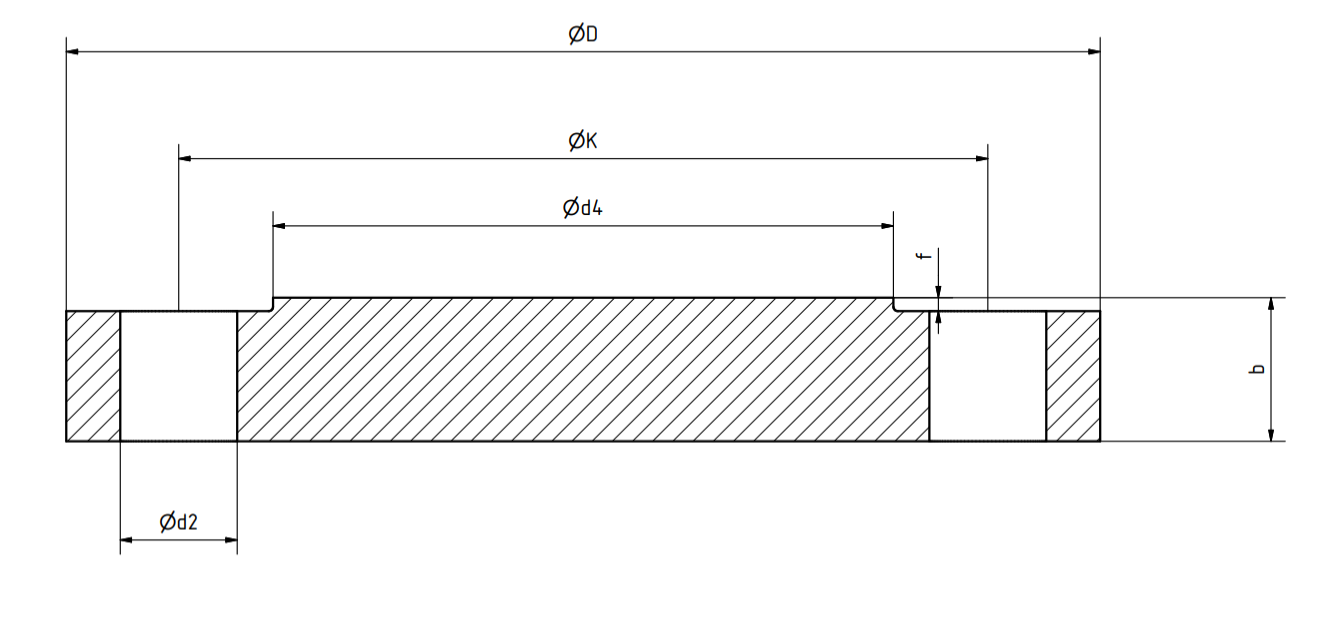
\includegraphics[scale=.25]{./images/vakkarima.png}
	\caption{Vakkarima előtervének rajza}
\end{figure}
\begin{align*}
	&D = \siunit{\karimaD}{\mm} \\
	&f = \siunit{\karimaf}{\mm} \\
	&d_4 = \siunit{\karimadfour}{\mm} \\
	&d_2 = \siunit{\karimadtwo}{\mm} \\
	&K = \siunit{\karimaK}{\mm} \\
	&b = \siunit{\karimab}{\mm} \\
\end{align*}
\begin{center}
	\begin{tabular}{l}
		$D$: vakkarima külső átmérő \siunit{}{\mm} \\
		$f$: kiugrás \siunit{}{\mm} \\
		$d_4$: tömítő felület külső átmérő \siunit{}{\mm} \\
		$d_2$: csavar lyukkör \siunit{}{\mm} \\
		$K$: csavarok középátmérő \siunit{}{\mm} \\
		$b$: vakkarima magassága \siunit{}{\mm} \\
	\end{tabular}
\end{center}

\newpage
\begin{figure}[hbt!]
	\centering
	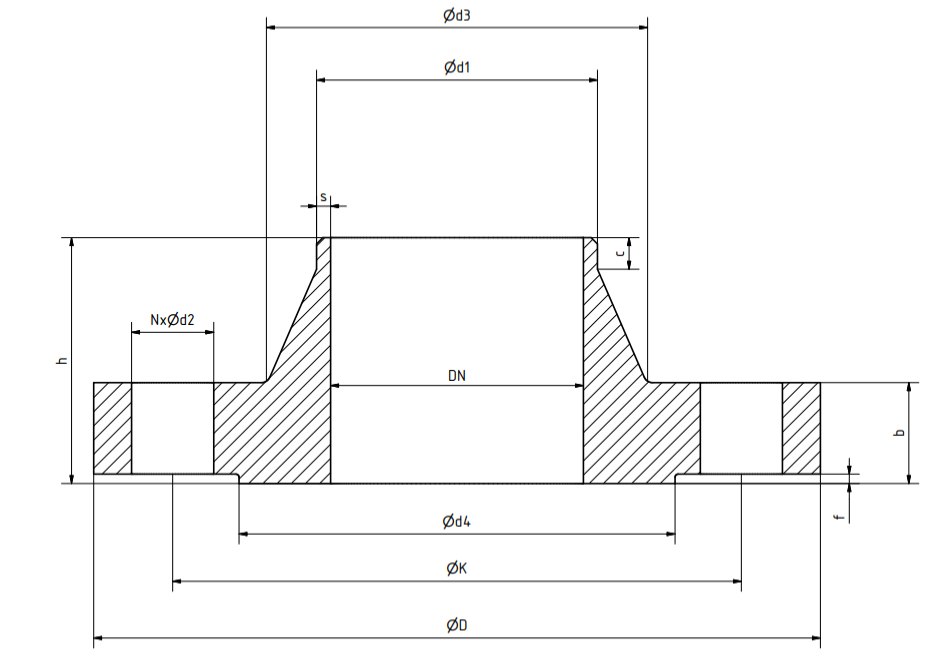
\includegraphics[scale=.61]{./images/karima.png}
	\caption{Karima előtervének rajza}
\end{figure}

\begin{minipage}{.45\linewidth}
	\begin{align*}
		&D = \siunit{\karimaD}{\mm} \\
		&f = \siunit{\karimaf}{\mm} \\
		&d_4 = \siunit{\karimadfour}{\mm} \\
		&d_2 = \siunit{\karimadtwo}{\mm} \\
		&s = \siunit{\karimas}{\mm} \\
		&N = \siunit{\karimaN}{db} \\
		&K = \siunit{\karimaK}{\mm} \\
		&b = \siunit{\karimab}{\mm} \\
		&d_3 = \siunit{\karimadthree}{\mm} \\
		&d_1 = \siunit{\karimadone}{\mm} \\
		&M = \text{M24} \\
		&h = \siunit{\karimah}{\mm}
	\end{align*}
\end{minipage}
\begin{minipage}{.5\linewidth}
	$D$: karima külső átmérő \siunit{}{\mm} \\
	$f$: kiugrás \siunit{}{\mm} \\
	$d_4$: tömítő felület külső átmérő \siunit{}{\mm} \\
	$d_2$: csavar lyukkör \siunit{}{\mm} \\
	$s$: falvastagság \siunit{}{\mm} \\
	$N$: csavarok \siunit{}{db} \\
	$K$: csavarok középátmérő \siunit{}{\mm} \\
	$b$: csavarok alap \\és tömítési sík távolság \siunit{}{\mm} \\
	$d_3$: kúp alsó átmérője \siunit{}{\mm} \\
	$d_1$: cső csatlakozás külső \siunit{}{\mm} \\
	$M$: csavar \siunit{}{\mm} \\
	$h$: karima magasság \siunit{}{\mm}
\end{minipage}

\newpage
\subsection[Minimális vastagság]{Minimális vastagság\protect\footnote{A feladathoz mellékelt segédletből származó számítások. (5. oldal)}}

A terhelés egy $d_t$ átmérőjű körön átadódó egyenletesen eloszlódó és feltehető hogy a törés egy egyenletes vonal mentén lesz. A vakkarimára ható erő a súlypontba lett felvéve ($y_k, y_d$).

\begin{equation}
	d_t = \frac{(d_1 - 2s) + d_4}{2} = \siunit{\karimaDt}{\mm}
\end{equation}

\begin{align}
	&y_k = \frac{k}{\pi} \\
	&y_d = \frac{2}{3} \frac{d_t}{\pi} \\
\end{align}

\begin{equation}
	b_{\text{min}} 
	= \frac{d_t}{2} \sqrt{\frac{3p_\text{ü}}{\sigma_{\text{hajl}}} \left(1-\frac{2}{3} \frac{d_t}{k}\right)} 
	= \siunit{\karimabmin}{\mm}
\end{equation}

\begin{align}
	&\sigma = 
	\frac{d_{t}^2}{4} 
	\frac{3p_{\text{ü}}}{b_{\text{min}}^2}
	\left(1-\frac{2}{3}\frac{d_t}{K}\right) = \mpa{\karimasigma} \\
	&n = \frac{\sigma_{\text{hajl}}}{\sigma} = \siunit{\kariman}{-}
\end{align}

\begin{center}
	\begin{tabular}{l}
		$d_t$: tőmítés középátmérő \siunit{}{\mm} \\
		$d_1$: cső csatlakozás külső \siunit{}{\mm} \\
		$s$: falvastagság \siunit{}{\mm} \\
		$d_4$: tömítő felület külső átmérő \siunit{}{\mm} \\
		$k$: csavar lyukkör \siunit{}{\mm} \\
		$y_k, y_d$: súlypont távolsága a vakkarima kör középpontjától \siunit{}{\mm} \\
		$b_\text{min}$: karima minimális vastagsága \siunit{}{\mm} \\
		$p_\text{ü}$: belső üzemi nyomás \siunit{}{\mm} \\
		$\sigma_\text{hajl}$: maximális hajlító feszültség \siunit{}{\mega\pascal} \\
		$\sigma$: hajlító feszültség minimális karima vastagsággal \siunit{}{\mega\pascal} \\
		$n$: biztonsági tényező \siunit{}{-} \\
	\end{tabular}
\end{center}
